\documentclass[runningheads]{llncs}

\usepackage{pdfpages}
\pdfminorversion=7
\usepackage{marvosym}
\usepackage[inline]{enumitem}
\usepackage{graphicx}
\usepackage[utf8]{inputenc}
\usepackage{times}
%\usepackage{hyperref}
%\usepackage{hyperxmp}
%\usepackage{url}

%\hypersetup{
   %pdflang={en},
   %colorlinks=false,
   %linkcolor=blue   
%}

\newcommand{\pcmember}[3]{\item #2 #1, #3}


\begin{document}

\title{5$^{\textrm{th}}$ Int'l MPM4CPS Workshop\\
{\small Multi-Paradigm Modeling for Cyber-Physical Systems}}

\vspace{-1cm}
\author{
   Moussa Amrani\inst{1}$^{,\textrm{\Letter}}$ \and
   Dominique Blouin\inst{2} \and
   Moharram Challenger\inst{3} \and
   Joeri Exelmans\inst{3} \and
   Randy Paredis\inst{3}$^{,\textrm{\Letter}}$ \and
   Robert Heinrich\inst{4}
}

\institute{
   University of Namur / NaDI, Belgium, \email{Moussa.Amrani@unamur.be} \and
   T\'el\'ecom Paris, Institut Polytechnique de Paris, France, \email{Dominique.Blouin@telecom-paris.fr} \and
   University of Antwerp - Flanders Make, Belgium,\\ \email{\{ Randy.Paredis, Joeri.Exelmans \} @uantwerpen.be}\and
   Karlsruhe Institute of Technology, Germany, \email{Robert.Heinrich@kit.edu}
}

%\author{Dominique Blouin}
%\affiliation{%
  %\institution{T\'el\'ecom Paris, Institut Polytechnique de Paris}
  %\city{Paris}
  %\country{France}}
%\email{Dominique.Blouin@telecom-paris.fr}
%
%\author{Moharram Challenger}
%\email{moharram.challenger@uantwerpen.be}
%\author{Joeri Exelmans}
%\email{Joeri.Exelman@uantwerpen.be}
%\author{Randy Paredis}
%\email{Randy.Paredis@uantwerpen.be}
%\affiliation{%
  %\institution{University of Antwerp - Flanders Make}
  %\city{Antwerp}
  %\country{Belgium}
%}
%
%\author{Robert Heinrich}
%\affiliation{%
  %\institution{Karlsruhe Institute of Technology}
  %\city{Karlsruhe}
  %\country{Germany}}
%\email{Robert.Heinrich@kit.edu}

\maketitle

\noindent
\textbf{Abstract}: 
\begin{small}
The networked combination of multi-physics systems (mechanical, 
electrical, hydraulic, biochemical, among others) with computational systems 
(control systems, signal processing, logical inference, planning, among others), 
often interacting with human actors, in uncertain environments, in a socio-economic 
context, has led to so-called Cyber-Physical Systems (CPS).
%
The CPS that are engineered today are reaching a previously unseen level of 
complexity.
To date, no unifying theory nor systematic design methods, techniques and tools 
exist for such systems.
Individual (mechanical, electrical, network or software) engineering disciplines 
only offer partial solutions.
Multi-Paradigm Modeling (MPM) proposes to \emph{model} every part and aspect of 
such complex systems \emph{explicitly}, at the most appropriate level(s) of 
abstraction, using the most appropriate modeling language(s)/formalism(s).
This includes the explicit modeling of the often complex engineering workflows.
Modular modeling language engineering, including model transformation and the 
study of modeling language semantics, are used to realize MPM, which has the 
potential to be an effective answer to the challenges of designing CPS.
%
This \textbf{fifth edition} is aimed at furthering the state-of-the-art as well as 
defining the future directions of this emerging research area by bringing together 
international experts in the field for an intense \textbf{one-day workshop}.
\end{small}




\section{Motivation}
\label{sec:Motivation}

%\subsection{Objectives and Scope}
%\label{sec:Objectives-Scope}

\noindent
\textbf{Objectives and Scope.}
%
Tackling the complexity involved in developing truly complex, designed systems 
is a topic of intense research and development.
In the past, system complexity has drastically increased once software components 
were introduced in the form of embedded systems, controlling physical parts of 
the system, and has only grown in CPS, where the networking aspect of the systems 
and their environment are also taken into account.
The complexity faced when engineering CPS is mostly due to the plethora of 
cross-disciplinary design alternatives and inter-domain interactions.
To date, no unifying theory nor system design methods, techniques, or tools to 
design, analyze, and ultimately deploy CPS exist.
Individual (physical systems, network, software) engineering disciplines offer 
only partial solutions and are no match for CPS complexity.



\emph{Multi-Paradigm Modeling (MPM)} offers a foundational framework for gluing the 
several disciplines together in a consistent way.
The inherent complexity of CPS is broken down into different levels of 
abstraction and views, each expressed in appropriate modeling formalisms.
MPM offers processes and tools that can integrate the views, abstractions and 
components that make up a CPS.

MPM encompasses many research topics: from language engineering (for DSLs, 
including their (visual) syntax and semantics), to processes to support multi-view 
and multi-abstraction modelling, simulation for full-system analysis, and deployment.
The added complexity that CPS bring compared to embedded and software-intensive 
systems requires consideration of how MPM techniques can be applied or adapted 
to these new applications, tying together multiple domains.
Many remaining research questions require answers from researchers in different 
domains, as well as a unified effort from researchers that work on supporting 
techniques and technologies.
The community needs a workshop setting to meet up and align past and future 
research activities.


\smallskip\noindent
\textbf{Workshop's Purpose.} During this Workshop, we want to bring together 
researchers and practitioners in the area of MPM (specifically applied to 
developing CPS) in order to identify possible points of synergy, common problems
and solutions, tool building aspects and the vision for the future of the area.
The goal is to organize a \textbf{highly interactive workshop}, with a significant 
portion of the Workshop dedicated to \textbf{discussions}.
\textbf{"Regular" Research papers} from academic and industry authors 
   will present novel research results on the Workshop's topics of interest. 
   We will encourage the submission of out-of-the-box presentations, which are 
   not deeply researched yet, but can lead to new insights, discussions, and 
   future collaborations.

As we already proposed last year, we will invite the submission of 
   \textbf{Exemplars}, i.e., typical yet relatively tractable use cases of CPS 
   demonstrating typical activities required for CPS Engineering, and explicitly
   detailing the underlying formalisms, languages and tools deployed to support 
   such activities, all expressed in a similar way to enable comparison and 
   extract CPS Engineering common practices and design patterns.

Those directions were not possible during the two previous editions due to the
virtual nature of the Workshop, but we hope to foster new topics and have small
groups discussing and brainstorming around the exemplars we collected so far 
(including the ones resulting from the previous edition).


%\subsection{Intended Audience}
%\label{sec:Audience}

\smallskip
\noindent
\textbf{Intended Audience.}
%
The intended audience includes researchers as well as practitioners who are 
interested in MPM techniques in the context of CPS development.
We expect to attract many attendees of earlier MPM-related events, those who 
contributed to the COST action, as well as a broader audience.
This includes researchers that work on the fundamentals of language 
engineering, (visual) modelling environment construction, (co-)simulation 
techniques, as well as tool builders and users of these tools.


%\subsection{Topics of Interest}
%\label{sec:ToI}

\smallskip
\noindent
\textbf{Topics of Interest.}
%
A list of topics of interest is given in the CfP available in Appendix.
Note that we have explicitly included \emph{classification} and \emph{exemplar} 
topics, as it is key to structure and discuss the future of MPM, and integrated 
broad topics related to \#MDE4SG (in the two last points).

%\begin{itemize}
   %\item Foundations of domain-specific modelling, with a particular focus on 
   %\emph{classifications} of the various dimensions around MPM (formalisms; processes;
   %related activities such as V\&V, deployment, calibration, etc.; tools, and 
   %methodologies);
   %\item Modelling language engineering, modular design of modelling languages, 
   %with a particular focus on de-/composition;
   %\item Co-simulation, coordination algorithms ensuring correct simulation results.
   %\item Digital twins of complex systems and their relationship to MPM techniques.
   %\item Applications of MPM techniques in automotive, aviation, manufacturing, etc.
   %\item MPM for (self-)adaptive systems
   %\item Machine Learning applied in an MPM context, Smart CPS
   %\item Social impacts processes in CPS, Large Data Management Modelling in CPS
%\end{itemize}

%\subsection{Relevance}
%\label{sec:Relevance}

\noindent
\textbf{Relevance.}
%
The MODELS conference is an ideal venue for organizing MPM4CPS since it brings 
together researchers that aim to advance the state-of-the-art in model-driven 
engineering and practitioners who have valuable application experiences to share.



%\subsection{Context}
%\label{sec:Context}

\smallskip
\noindent
\textbf{Context.}
%
The MPM community has been actively researching new techniques for system design 
for over a decade, through many related events.
One-week Computer Automated Multi-Paradigm Modeling (CAMPaM) workshops have been 
organized yearly since 2004 at McGill University’s Bellairs campus, Barbados. 
Additionally, the International Summer School on Domain-Specific Languages - 
Theory and Practice (DSM-TP), focused on the education of language engineering 
techniques, and has been organized since 2009.
Its target audience includes Ph.D. students, researchers, and software industry 
professionals.
Most recently, a European Cooperation in Science and Technology (COST) research 
network has been active since 2015 on the use of MPM techniques for designing 
CPS, bringing together 29 European partner countries\footnote{https://www.cost.eu/actions/IC1404/ 
and http://mpm4cps.eu/}.
The chair and co-chair of this network (Hans Vangheluwe and Vasco Amaral) are 
members of the steering committee for this workshop.

The first edition of the workshop has lead to the preparation of a theme section
on the topic of MPM4CPS for the SoSyM journal (which has been finally published%
\footnote{ https://link.springer.com/article/10.1007/s10270-021-00882-1}).
The second and third editions were operated fully online, and therefore have been
reduced to half-day workshops consisting solely of paper presentations, albeit with
longer discussion periods (typically, 10-15 minutes after each presentation), and
each paper presentation session still attracted ca. 20-25 participants with lively,
interesting discussions. Because of the virtual/online nature of these editions,
hosting an interactive/''brainstorming'' session was difficult, but we strongly
believe those sessions are at the heart of MPM4CPS, and will attract enough
participants (around 10, not counting the organisation members).

All these initiatives, as well as the success during the online editions, 
demonstrate both the continued relevance of the topic, and the 
potential impact of a new edition of the workshop.



%\subsection{Needs}
%\label{sec:Needs}

\smallskip
\noindent
\textbf{Needs.}
%
The MPM4CPS workshop (series) follows the successful series of nine MPM workshops that 
were organized as part of the MODELS conference during the years 2006 through 2015.
These workshops attracted many participants in the past, and we saw that the topic
is still relevant, since the previous editions attracted many submissions and lively discussions.
These two reasons make this workshop worth organizing at MODELS this year.

Historically, GeMoC and EXE, now merged into the MLE (Modeling Language 
Engineering and Execution), were the closest workshops planned to be organised 
in MoDELS this year. They focus mainly on two topics: the globalization of
modeling techniques, which include techniques and processes to create and
integrate heterogeneous languages, and the execution, animation and debugging
of modeling languages. While both are concerned with specific aspects of 
\emph{software} language engineering, MPM includes modeling languages for 
physical domains (e.g., electrical, mechanical, etc.) that require 
continuous-time solvers for simulation, and clean integration with other (SW/HW) 
languages.
MPM4CPS further differentiates from those workshops by focusing on CPS. 
We believe that both workshops can strengthen each other by focusing on different 
(specialized) aspects of challenges within the MODELS community.

The challenges to design and develop CPS, with a focus on MPM techniques as a 
foundational framework for supporting the multi-domain models, tools, and 
processes are fundamental enough to warrant a focused workshop.

\section{Organisation Details}
\label{sec:Organisation}

We are joined by two new organising members, Joeri Exelmans and Randy Paredis, 
who will take care of the Publicity and Website, paired with more senior organisers.

The \textbf{expected} PC is given in the CfP in Appendix.
We request that MPM4CPS be run on its own as we plan half a day of discussions.
We can merge with another workshop if this is a condition from the organization 
and the topics are similar enough.

\medskip
\noindent
\textbf{Moussa Amrani} obtained his Ph.D. in 2013 from the University of Luxembourg. 
He is currently a postdoctoral researcher at the University of Namur and the Namur Digital Institute in Belgium. 
He is (co-)author of over 50 papers on MDE, IoT and formal verification published in international conferences (MODELS, SLE, ECMFA, ASE, ETAPS, NFM, CAiSE, \ldots) and journals (SoSyM, JSS, TSE, ToSEM, JoT, IST, ComLan, \ldots). He co-founded and co-organized the VoLT workshop at MoDELS from its inception in 2013, and co-organised
the previous editions of the MPM4CPS Workshop.

\medskip
\noindent
\textbf{Dominique Blouin} is a research engineer at Telecom Paris, Institut Polytechnique Paris 
(France). He obtained an M.Sc. in Physics (Canada) and a Ph.D. in Computer Science (France) in 2013. He worked for many years in industry as a software architect and was the vice-chair of the Foundational Aspects Working Group in the MPM4CPS COST Action. He has been an active member of the SAE AADL standardization committee for the past 10 years. His research interests are MPM, model management, model transformation and (bi-directional) synchronization, requirements engineering, CPS.

\medskip
\noindent
\textbf{Moharram Challenger} is a research professor at the University of Antwerp, Belgium. He was the CTO of a software company involved-in/leading several national and international software intensive projects. He has served as an organisation committee member for SummerSim'20, ICSMM'20, AnnSim'21, IWCPS@FedCSIS'21, and AMSC'21. Also, he played the role of co-chair for several workshops organised in MoDELS and STAF 2020-21 (MDE-Intelligence, MPM4CPS, MDE4IoT, SERP4IoT, SEDES, MESS, EMAS, etc.).

\medskip
\noindent
\textbf{Joeri Exelmans} is a Ph.D. student at the University of Antwerp, Belgium, and has worked on a Flanders Make project aiming to facilitate collaboration in complex engineering workflows. His research interests are the engineering of hybrid modeling languages, model versioning, and inconsistency management and traceability in complex engineering workflows.

\medskip
\noindent
\textbf{Randy Paredis} is a Ph.D. student at the University of Antwerp, Belgium, and is exploring architectures and frameworks for model-based design of Digital Twins within the context of Industry 4.0. His research interests are multi-paradigm modelling, using DEVS as a common denominator for discrete-event modelling languages, and co-simulation.


\medskip
\noindent
\textbf{Robert Heinrich} holds a Ph.D. from Heidelberg University, and is head of the Quality-driven System Evolution research group at KIT. His research interests include modularization
and composition of model-based analysis for performance, confidentiality and maintainability, etc. applied to information systems, business processes and automated production systems. One core asset of his work is the Palladio software architecture simulator. He is involved in the organization committees of several international conferences, established and organized various workshops, is reviewer for international premium journals (IEEE TSE and IEEE Software), and academic funding agencies.


\section{Workshop Format}
\label{sec:Format}

\begin{description}
   \item[Deadlines \& Paper Format] Cf. CfP in Appendix
   
   \item[Evaluation Process] At least three reviewers will evaluate each submission.
   Full research papers will be reviewed using standard scientific criteria: alignment 
   with the workshop topic(s), novelty, evaluation, and ability to generate discussion.
   Short papers will be evaluated based on their likelihood to spark lively 
   discussions.

   \item[Intended Workshop Format] In the ideal case of a full day workshop, we 
   will host two keynotes, ideally one from academia and the other from industry
   (depending on how people are available). 
   A morning keynote will set the stage for the rest of the day, followed by 
   paper presentations. A second keynote after the lunch break will set the 
   discussion around exemplar presentations and new and provocative ideas,
   which will foster discussions and out-of-the-box ideas. Each talk throughout the
   day will be followed by discussions.
   The afternoon will reserve time to discuss the examplars, by starting discussions
   around identifiable patterns, common practices, popular formalisms/languages/tools, etc. 
   The workshop will end with a wrap-up discussion to formulate the workshop's 
   conclusion, identify open challenges, and outline future work.
   A summarizing publication will be included in the proceedings. 
   Depending on the quality of papers/discussions, we may organise a Special Issue
   based on invitations (this/previous edition(s)) and open call.
   
   \item[(Expected) Participants Number] 25-35 (similar to previous editions.)
   
   \item[Equipment] Whiteboard + Slide Projection
\end{description}

%\subsection{Deadlines \& Paper Format: cf. CfP}
%\label{sec:Deadlines-Format}
%
%\subsection{Evaluation Process}
%\label{sec:EvaluationProcess}
%
%At least three reviewers will evaluate each submission.
%Full research papers will be reviewed using standard scientific criteria: alignment 
%with the workshop topic(s), novelty, evaluation, and ability to generate discussion.
%Short papers will be evaluated based on their likelihood to spark lively 
%discussions at the workshop.
%
%\subsection{Intended Workshop Format}
%\label{sec:Format-Workshop}
%
%In the ideal case of a full day workshop, we will host two keynotes, ideally 
%one from academia and the other from industry (depending on how people are 
%available). A morning keynote will set the stage for the rest of the day, 
%followed by paper presentations. A second keynote after the lunch break
%will set the discussion around exemplar presentations and new and provocative ideas,
%which will foster discussions and out-of-the-box ideas. Each talk throughout the
%day will be followed by discussions.
%
%The afternoon will reserve time to discuss the examplars, by starting discussions
%around identifiable patterns, common practices, popular formalisms/languages/tools, etc. 
%The workshop will end with a wrap-up discussion to formulate the workshop's 
%conclusion, identify open challenges, and outline future work.
%A summarizing publication will be included in the proceedings.
%
%\subsection{(Expected) Participants Number: 25-35 (similar to previous editions.)}
%
%\subsection{Equipment: Whiteboard}




\section{Additional Material}
\label{sec:Appendix}

A draft \textbf{Call for Paper} is attached as Appendix.
The \textbf{URL} is already available and will be completed when new information
becomes available.

\noindent
\url{\texttt{http://msdl.uantwerpen.be/conferences/MPM4CPS/2022}}

\newpage
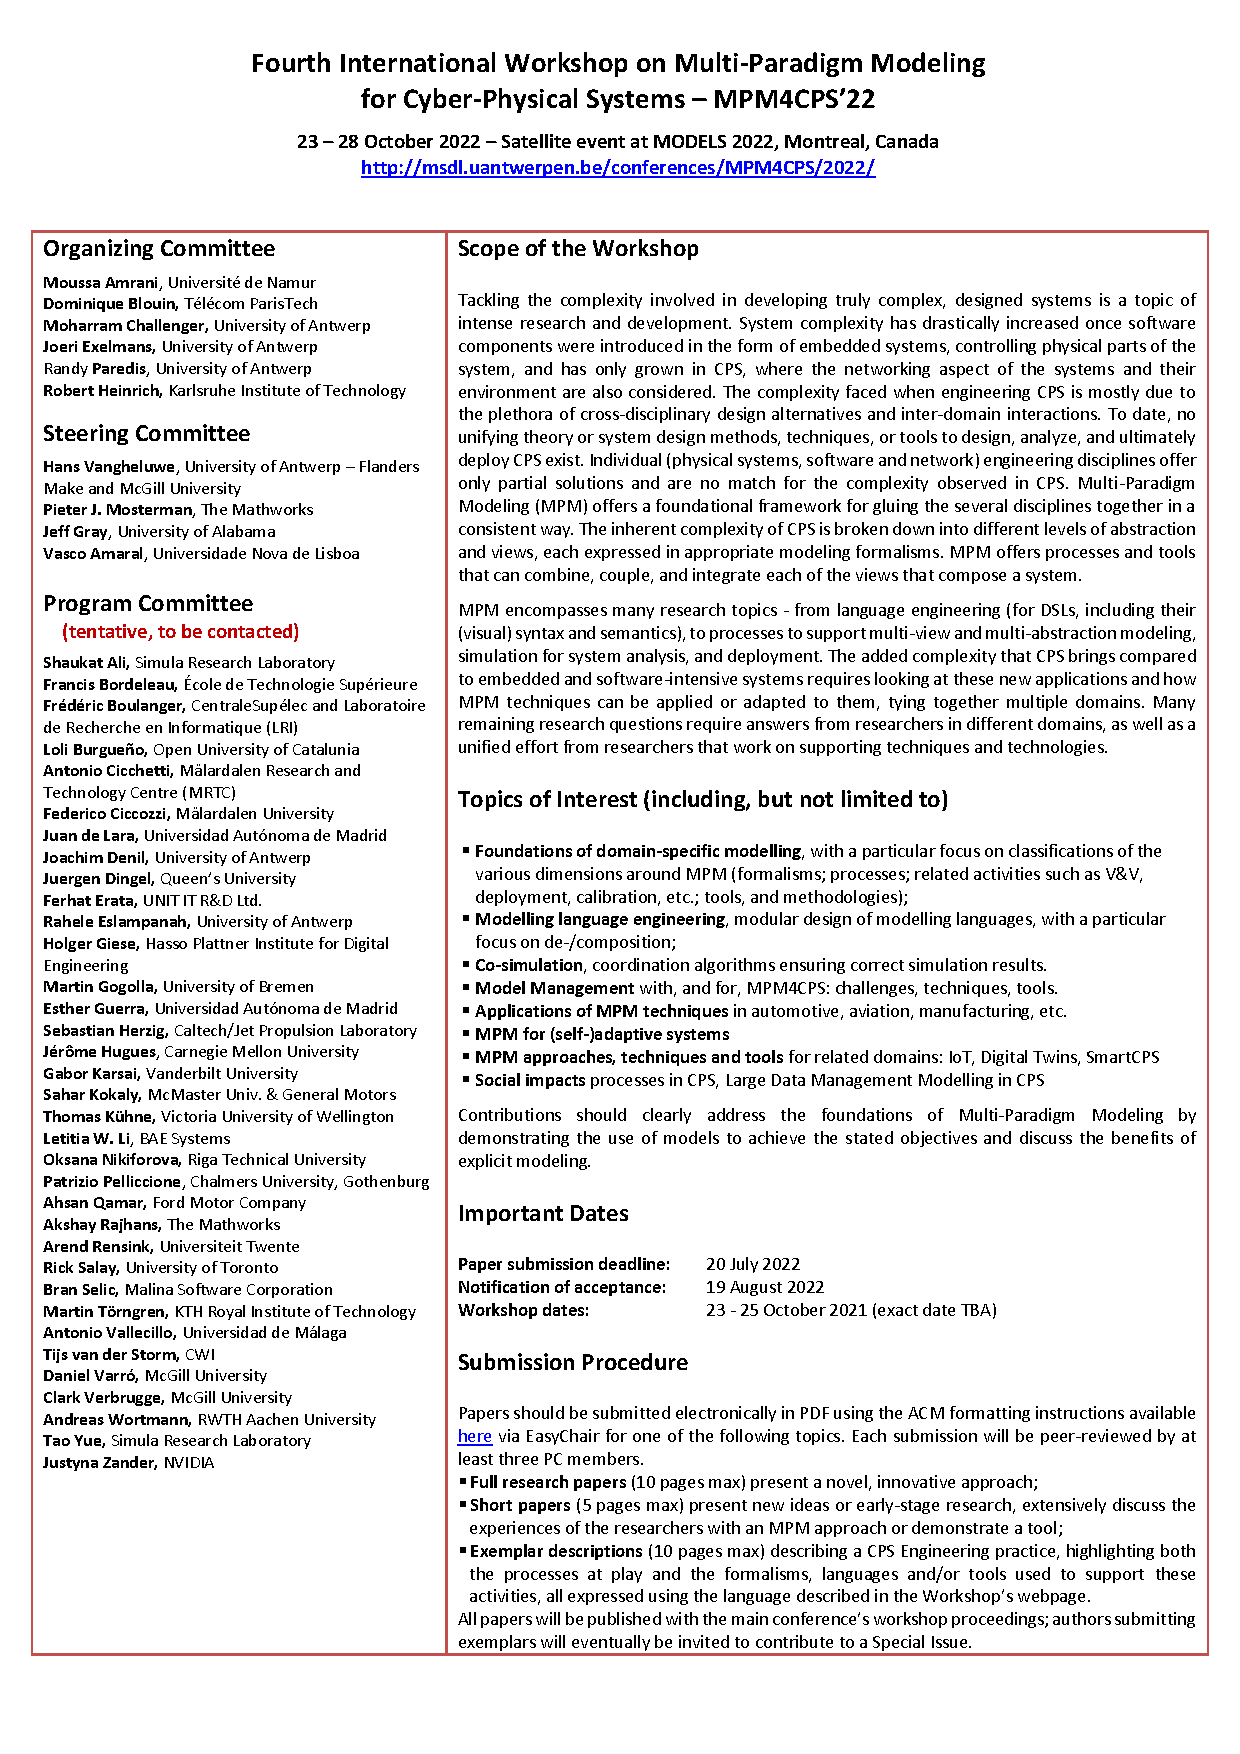
\includepdf{cfp/MPM4CPS22-CfP.pdf}

https://www.overleaf.com/project/623336d3413bc0d63cf9c1d2

\end{document}